% ============================================================
% Poster: Starlink-Primary Resilient Gateway Reference Lab
% Tamaño: doble carta (tabloide) 17in x 11in, horizontal
% Compilar: pdflatex diagrama-lab-doble-carta.tex
% PNG 300dpi: pdftoppm -png -r 300 diagrama-lab-doble-carta.pdf
% Fuente de contenido: ../03-arquitectura.md
% ============================================================
\documentclass[11pt]{article}
\usepackage[paperwidth=17in,paperheight=11in,margin=0in]{geometry}
\usepackage[T1]{fontenc}
\usepackage[utf8]{inputenc}
\usepackage[scaled=.96]{helvet}
\renewcommand{\familydefault}{\sfdefault}
\usepackage{xcolor}
\usepackage{tikz}
\usetikzlibrary{calc,arrows.meta,decorations.pathmorphing,positioning}
\pagestyle{empty}

% ---- Paleta (misma del pitch ejecutivo) --------------------
\definecolor{AccentBlue}{HTML}{3A83C2}
\definecolor{PrimaryBlue}{HTML}{1B5A8F}
\definecolor{Slate}{HTML}{273140}
\definecolor{Muted}{HTML}{5A6470}
\definecolor{DigiGreen}{HTML}{5B9E31}
\definecolor{Fase2Orange}{HTML}{D97706}
\definecolor{RFViolet}{HTML}{7A4FA0}
\definecolor{PaperBG}{HTML}{FBFCFE}

% ---- Estilos de enlace -------------------------------------
\tikzset{
  wanstar/.style={line width=2.6pt, PrimaryBlue},
  wan5g/.style={line width=2pt, AccentBlue},
  fabric/.style={line width=2.6pt, DigiGreen},
  mgmt/.style={line width=1.1pt, Muted, densely dotted},
  oob/.style={line width=1.8pt, Fase2Orange, dashed},
  rf/.style={line width=1.2pt, RFViolet, decorate,
             decoration={snake, amplitude=.45mm, segment length=2.2mm, post length=1mm}},
  beam/.style={line width=.9pt, AccentBlue!75, densely dotted},
  caption/.style={font=\small, text=Slate, align=center},
  subcap/.style={font=\footnotesize, text=Muted, align=center},
  linklab/.style={font=\footnotesize\bfseries, text=Slate, fill=PaperBG, inner sep=1.5pt, align=center},
}

% ============ ICONOS DE PRODUCTO (pics) =====================
\tikzset{
  % --- Satélite Starlink ---
  pics/satellite/.style={code={
    \fill[AccentBlue!65, draw=Slate, line width=.5pt] (-0.36,-0.05) rectangle (-0.13,0.05);
    \fill[AccentBlue!65, draw=Slate, line width=.5pt] (0.13,-0.05) rectangle (0.36,0.05);
    \fill[Slate] (-0.10,-0.07) rectangle (0.10,0.07);
    \draw[Slate, line width=.7pt] (-0.13,0) -- (-0.10,0) (0.10,0) -- (0.13,0);
  }},
  % --- Antena plana Starlink Gen 3 sobre soporte ---
  pics/dish/.style={code={
    \draw[line width=2pt, Slate, line cap=round] (0.06,-0.06) -- (0.14,-0.52);
    \draw[line width=2pt, Slate, line cap=round] (-0.16,-0.52) -- (0.44,-0.52);
    \begin{scope}[rotate=18]
      \fill[white, draw=Slate, line width=1.4pt, rounded corners=3pt] (-0.62,-0.40) rectangle (0.62,0.40);
      \fill[AccentBlue!14, rounded corners=2pt] (-0.54,-0.32) rectangle (0.54,0.32);
      \fill[Slate] (0,0) circle (0.035);
    \end{scope}
  }},
  % --- Torre celular ---
  pics/celltower/.style={code={
    \draw[Slate, line width=1.1pt] (-0.24,-0.72) -- (0,0.38) -- (0.24,-0.72);
    \draw[Slate, line width=.6pt] (-0.16,-0.36) -- (0.16,-0.36) (-0.20,-0.55) -- (0.20,-0.55)
      (-0.16,-0.36) -- (0.20,-0.55) (0.16,-0.36) -- (-0.20,-0.55)
      (-0.11,-0.14) -- (0.11,-0.14) (-0.11,-0.14) -- (0.16,-0.36) (0.11,-0.14) -- (-0.16,-0.36);
    \fill[Slate] (-0.035,0.30) rectangle (0.035,0.52);
    \draw[AccentBlue, line width=.9pt] (0.10,0.46) arc (-40:40:0.16);
    \draw[AccentBlue, line width=.9pt] (0.17,0.38) arc (-40:40:0.28);
    \draw[AccentBlue, line width=.9pt] (-0.10,0.46) arc (220:140:0.16);
    \draw[AccentBlue, line width=.9pt] (-0.17,0.38) arc (220:140:0.28);
  }},
  % --- Router Digi IX40 ---
  pics/router/.style={code={
    \draw[line width=1.9pt, Slate, line cap=round] (-0.82,0.42) -- (-0.98,0.95);
    \draw[line width=1.9pt, Slate, line cap=round] (0.82,0.42) -- (0.98,0.95);
    \fill[Slate] (-0.98,0.95) circle (0.045) (0.98,0.95) circle (0.045);
    \fill[white, draw=PrimaryBlue, line width=1.6pt, rounded corners=4pt] (-1.05,-0.42) rectangle (1.05,0.42);
    \node[font=\small\bfseries, text=PrimaryBlue] at (0,0.14) {DIGI IX40-05};
    \foreach \px in {-0.78,-0.55,-0.32,-0.09}{
      \draw[Slate, line width=.8pt] (\px,-0.30) rectangle ++(0.16,0.14);}
    \node[font=\tiny, text=Muted] at (0.42,-0.23) {SFP};
    \draw[DigiGreen, line width=.9pt] (0.30,-0.31) rectangle ++(0.24,0.15);
    \fill[DigiGreen] (0.70,-0.16) circle (0.030) (0.80,-0.16) circle (0.030) (0.90,-0.16) circle (0.030);
    \draw[Slate, line width=.8pt] (0.66,-0.31) rectangle ++(0.28,0.10);
  }},
  % --- Nube (DRM) ---
  pics/cloudpic/.style={code={
    \path[fill=white, draw=PrimaryBlue, line width=1.6pt]
      (-0.78,0) .. controls (-1.08,0.02) and (-1.04,0.44) .. (-0.66,0.44)
      .. controls (-0.62,0.74) and (-0.16,0.80) .. (0.02,0.58)
      .. controls (0.24,0.82) and (0.72,0.70) .. (0.72,0.40)
      .. controls (1.06,0.38) and (1.08,0.02) .. (0.76,0)
      -- cycle;
  }},
  % --- Servidor rack ---
  pics/server/.style={code={
    \fill[white, draw=Slate, line width=1.2pt, rounded corners=2pt] (-0.40,-0.52) rectangle (0.40,0.52);
    \foreach \sy in {0.18,-0.14,-0.46}{
      \draw[Slate, line width=.7pt] (-0.40,\sy+0.30) -- (0.40,\sy+0.30);
      \fill[DigiGreen] (-0.28,\sy+0.15) circle (0.032);
      \draw[Muted, line width=.7pt] (-0.10,\sy+0.15) -- (0.28,\sy+0.15);}
  }},
  % --- SoM ConnectCore (chip) ---
  pics/som/.style={code={
    \foreach \pp in {-0.24,-0.08,0.08,0.24}{
      \draw[Slate, line width=1pt] (\pp,0.34) -- (\pp,0.46) (\pp,-0.34) -- (\pp,-0.46)
                                   (0.34,\pp) -- (0.46,\pp) (-0.34,\pp) -- (-0.46,\pp);}
    \fill[white, draw=Slate, line width=1.3pt, rounded corners=1.5pt] (-0.34,-0.34) rectangle (0.34,0.34);
    \fill[DigiGreen!22, draw=DigiGreen, line width=.9pt] (-0.20,-0.20) rectangle (0.20,0.20);
    \node[font=\tiny\bfseries, text=PrimaryBlue] at (0,0.02) {MP255};
  }},
  % --- Módulo XBee (PCB con antena) ---
  pics/xbeemod/.style={code={
    \fill[AccentBlue!16, draw=PrimaryBlue, line width=1.2pt, rounded corners=2pt] (-0.26,-0.30) rectangle (0.26,0.24);
    \draw[PrimaryBlue, line width=1.1pt] (0,0.24) -- (0,0.42);
    \fill[PrimaryBlue] (0,0.44) circle (0.035);
    \node[font=\scriptsize\bfseries, text=PrimaryBlue] at (0,-0.04) {X};
  }},
  % --- Gateway XBee Hive ---
  pics/hive/.style={code={
    \fill[white, draw=PrimaryBlue, line width=1.3pt, rounded corners=3pt] (-0.42,-0.26) rectangle (0.42,0.26);
    \draw[PrimaryBlue, line width=1.2pt, line cap=round] (0.30,0.26) -- (0.42,0.58);
    \fill[PrimaryBlue] (0.42,0.58) circle (0.035);
    \node[font=\scriptsize\bfseries, text=PrimaryBlue] at (-0.02,0.02) {HIVE};
    \fill[DigiGreen] (-0.28,-0.14) circle (0.028) (-0.18,-0.14) circle (0.028);
  }},
  % --- Sensor físico ---
  pics/sensorpic/.style={code={
    \fill[white, draw=RFViolet, line width=1.2pt] (0,0) circle (0.26);
    \draw[RFViolet, line width=1pt] (0,-0.08) -- (0,0.12);
    \fill[RFViolet] (0,-0.11) circle (0.055);
  }},
  % --- Consola OOB Opengear OM1304 ---
  pics/consoleserver/.style={code={
    \fill[white, draw=Fase2Orange, line width=1.4pt, rounded corners=2.5pt] (-0.72,-0.20) rectangle (0.72,0.20);
    \foreach \px in {-0.56,-0.38,-0.20,-0.02}{
      \draw[Slate, line width=.8pt] (\px,-0.07) rectangle ++(0.13,0.13);}
    \fill[Fase2Orange] (0.30,0.0) circle (0.030);
    \node[font=\tiny\bfseries, text=Fase2Orange] at (0.48,0.0) {OM};
  }},
  % --- Switch ---
  pics/switchpic/.style={code={
    \fill[white, draw=DigiGreen, line width=1.3pt, rounded corners=2.5pt] (-0.52,-0.19) rectangle (0.52,0.19);
    \draw[-{Stealth[length=4pt]}, DigiGreen, line width=1pt] (-0.36,0.05) -- (0.10,0.05);
    \draw[-{Stealth[length=4pt]}, DigiGreen, line width=1pt] (0.36,-0.06) -- (-0.10,-0.06);
  }},
  % --- PDU / UPS ---
  pics/pdu/.style={code={
    \fill[white, draw=Slate, line width=1.2pt, rounded corners=2pt] (-0.20,-0.46) rectangle (0.20,0.46);
    \fill[Slate!85] (-0.06,0.20) -- (0.07,0.20) -- (0.00,0.02) -- (0.09,0.02) -- (-0.05,-0.22) -- (0.00,-0.04) -- (-0.09,-0.04) -- cycle;
    \draw[Slate, line width=.8pt] (0,-0.33) circle (0.062);
    \fill[Slate] (-0.022,-0.33) circle (0.014) (0.022,-0.33) circle (0.014);
  }},
  % --- Contenedor (Digi Container) ---
  pics/containerpic/.style={code={
    \fill[white, draw=AccentBlue, line width=1.2pt, rounded corners=1.5pt] (-0.34,-0.18) rectangle (0.34,0.18);
    \foreach \px in {-0.20,-0.07,0.06,0.19}{
      \draw[AccentBlue, line width=.8pt] (\px,-0.12) -- (\px,0.12);}
  }},
}

\begin{document}
\noindent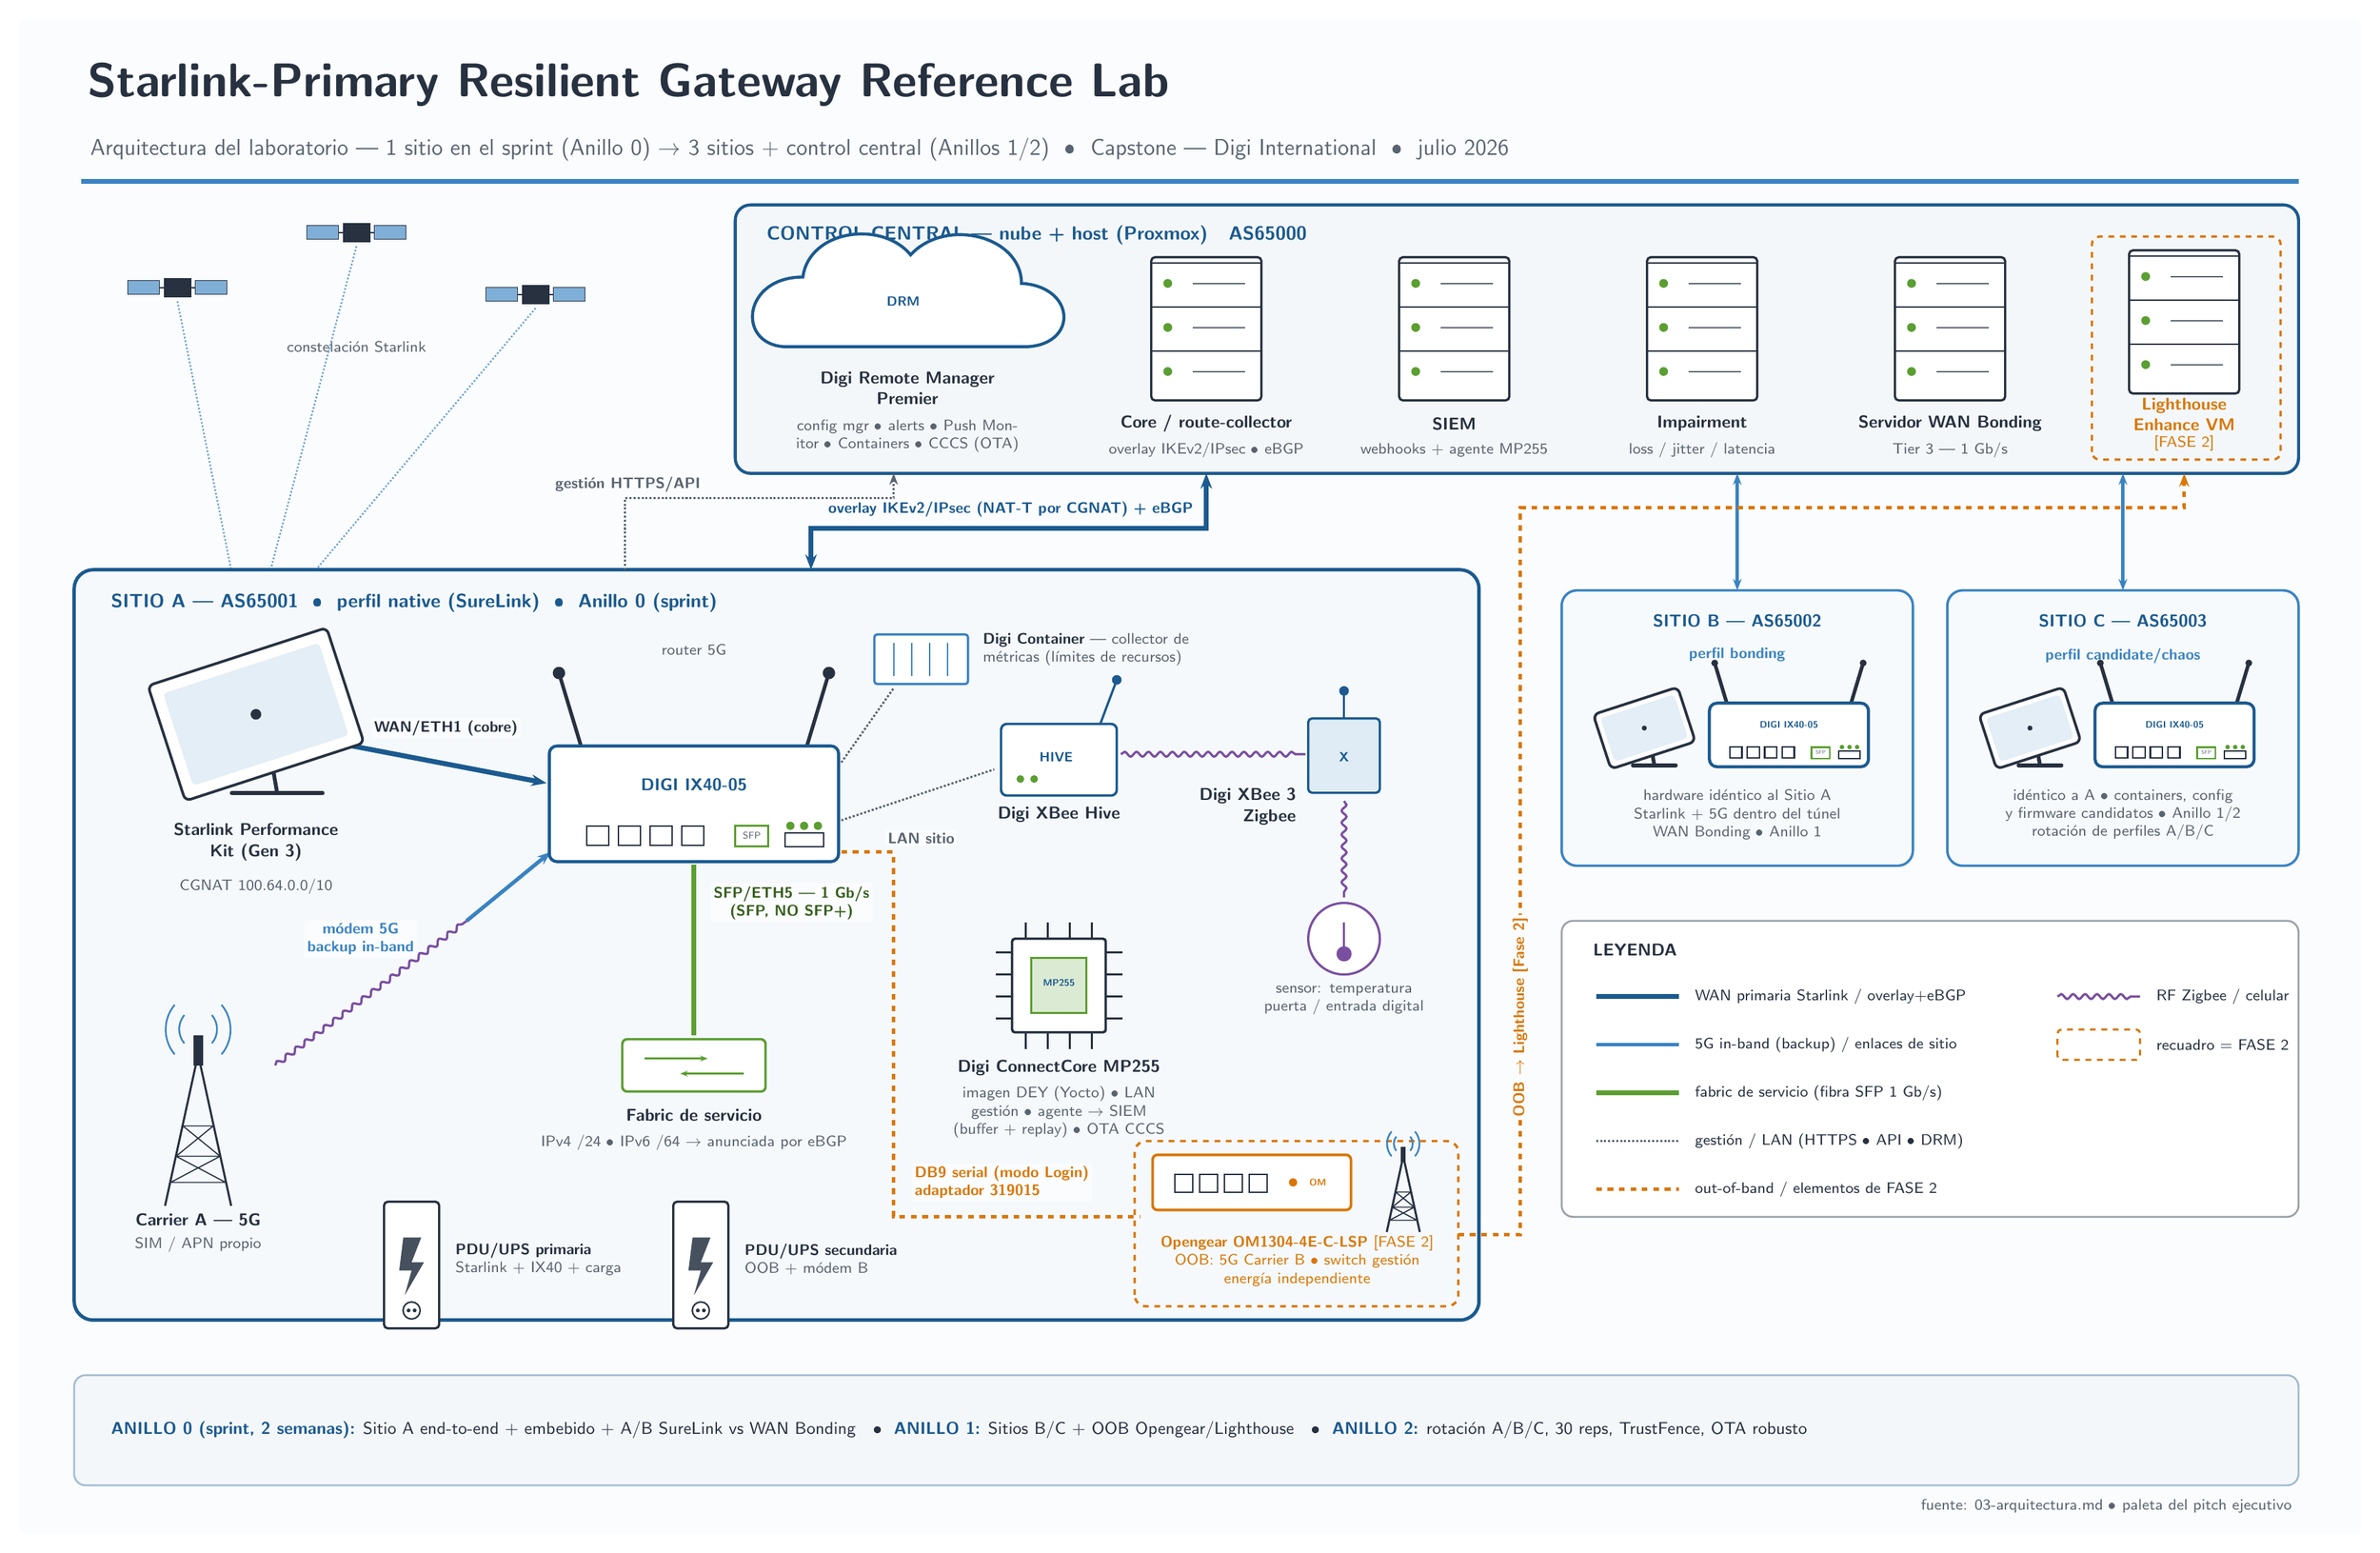
\begin{tikzpicture}[x=1in, y=1in]
  % ================= FONDO =================
  \fill[PaperBG] (0,0) rectangle (17,11);

  % ================= TÍTULO =================
  \node[anchor=west, font=\fontsize{30}{34}\selectfont\bfseries, text=Slate] at (0.45,10.52)
    {Starlink-Primary Resilient Gateway Reference Lab};
  \node[anchor=west, font=\large, text=Muted] at (0.47,10.05)
    {Arquitectura del laboratorio --- 1 sitio en el sprint (Anillo 0) $\rightarrow$ 3 sitios + control central (Anillos 1/2) \ \textbullet\ \ Capstone --- Digi International \ \textbullet\ \ julio 2026};
  \draw[AccentBlue, line width=2.5pt] (0.45,9.82) -- (16.55,9.82);

  % ================= CONSTELACIÓN STARLINK =================
  \pic at (1.15,9.05) {satellite};
  \pic at (2.45,9.45) {satellite};
  \pic at (3.75,9.00) {satellite};
  \node[subcap] at (2.45,8.62) {constelaci\'on Starlink};
  \draw[beam] (1.15,8.95) -- (1.62,6.60);
  \draw[beam] (2.45,9.35) -- (1.72,6.60);
  \draw[beam] (3.75,8.90) -- (1.82,6.60);

  % ================= CONTROL CENTRAL =================
  \fill[PrimaryBlue!5, draw=PrimaryBlue, line width=1.6pt, rounded corners=8pt] (5.2,7.7) rectangle (16.55,9.65);
  \node[anchor=north west, font=\normalsize\bfseries, text=PrimaryBlue] at (5.38,9.55)
    {CONTROL CENTRAL --- nube + host (Proxmox) \ \ AS65000};

  % DRM Premier
  \pic[scale=1.15] at (6.45,8.62) {cloudpic};
  \node[font=\scriptsize\bfseries, text=PrimaryBlue] at (6.42,8.95) {DRM};
  \node[caption, font=\small\bfseries] at (6.45,8.32) {Digi Remote Manager\\Premier};
  \node[subcap, text width=1.9in] at (6.45,7.97) {config mgr \textbullet\ alerts \textbullet\ Push Monitor \textbullet\ Containers \textbullet\ CCCS (OTA)};

  % Core / route-collector
  \pic at (8.62,8.75) {server};
  \node[caption, font=\small\bfseries] at (8.62,8.06) {Core / route-collector};
  \node[subcap] at (8.62,7.87) {overlay IKEv2/IPsec \textbullet\ eBGP};

  % SIEM
  \pic at (10.42,8.75) {server};
  \node[caption, font=\small\bfseries] at (10.42,8.06) {SIEM};
  \node[subcap] at (10.42,7.87) {webhooks + agente MP255};

  % Impairment
  \pic at (12.22,8.75) {server};
  \node[caption, font=\small\bfseries] at (12.22,8.06) {Impairment};
  \node[subcap] at (12.22,7.87) {loss / jitter / latencia};

  % WAN Bonding server
  \pic at (14.02,8.75) {server};
  \node[caption, font=\small\bfseries] at (14.02,8.06) {Servidor WAN Bonding};
  \node[subcap] at (14.02,7.87) {Tier 3 --- 1 Gb/s};

  % Lighthouse (fase 2)
  \draw[Fase2Orange, dashed, line width=1.2pt, rounded corners=4pt] (15.05,7.80) rectangle (16.42,9.42);
  \pic at (15.72,8.80) {server};
  \node[caption, font=\small\bfseries, text=Fase2Orange] at (15.72,8.13) {Lighthouse\\Enhance VM};
  \node[subcap, text=Fase2Orange] at (15.72,7.92) {[FASE 2]};

  % ================= SITIO A =================
  \fill[AccentBlue!5, draw=PrimaryBlue, line width=1.8pt, rounded corners=10pt] (0.4,1.55) rectangle (10.6,7.0);
  \node[anchor=north west, font=\normalsize\bfseries, text=PrimaryBlue] at (0.62,6.88)
    {SITIO A --- AS65001 \ \textbullet\ \ perfil \textsc{native} (SureLink) \ \textbullet\ \ Anillo 0 (sprint)};

  % ---- ENLACES PRIMERO (quedan debajo de iconos y etiquetas) ----
  % WAN primaria: dish -> IX40
  \draw[wanstar, -{Stealth[length=8pt]}] (2.42,5.72) -- (3.83,5.45);
  % 5G backup: torre -> IX40
  \draw[rf] (1.86,3.40) -- (3.25,4.45);
  \draw[wan5g, -{Stealth[length=7pt]}] (3.25,4.45) -- (3.86,4.95);
  % fiber SFP/ETH5
  \draw[fabric] (4.90,4.86) -- (4.90,3.62);
  % LAN sitio a Hive
  \draw[mgmt] (5.97,5.18) -- (7.08,5.55);
  % container link
  \draw[mgmt] (5.97,5.60) -- (6.35,6.14);
  % serial DB9 IX40 -> OM1304 (fase 2)
  \draw[oob] (5.97,4.95) -- (6.35,4.95) -- (6.35,2.30) -- (8.14,2.30);
  % RF hive -> xbee -> sensor
  \draw[rf] (8.00,5.66) -- (9.34,5.66);
  \draw[rf] (9.62,5.32) -- (9.62,4.62);

  % ---- ICONOS Y ETIQUETAS ----
  % Starlink kit
  \pic[scale=1.1] at (1.72,5.95) {dish};
  \node[caption, font=\small\bfseries] at (1.72,5.02) {Starlink Performance\\Kit (Gen 3)};
  \node[subcap] at (1.72,4.70) {CGNAT 100.64.0.0/10};
  \node[linklab] at (3.10,5.85) {WAN/ETH1 (cobre)};

  % Torre Carrier A
  \pic at (1.30,3.10) {celltower};
  \node[caption, font=\small\bfseries] at (1.30,2.28) {Carrier A --- 5G};
  \node[subcap] at (1.30,2.10) {SIM / APN propio};
  \node[linklab, text=AccentBlue] at (2.48,4.32) {m\'odem 5G\\backup in-band};

  % Router IX40
  \pic at (4.90,5.30) {router};
  \node[subcap] at (4.90,6.42) {router 5G};

  % Digi Container
  \pic at (6.55,6.35) {containerpic};
  \node[subcap, anchor=west, align=left] at (6.95,6.42) {\textbf{\textcolor{Slate}{Digi Container}} --- collector de\\m\'etricas (l\'imites de recursos)};

  % Etiquetas fiber / LAN
  \node[linklab, anchor=west, text=DigiGreen!60!black] at (5.02,4.58) {SFP/ETH5 --- 1 Gb/s\\(SFP, \textbf{NO} SFP+)};
  \node[linklab, text=Muted] at (6.55,5.05) {LAN sitio};

  % Fabric de servicio
  \pic at (4.90,3.40) {switchpic};
  \node[caption, font=\small\bfseries] at (4.90,3.04) {Fabric de servicio};
  \node[subcap] at (4.90,2.84) {IPv4 /24 \textbullet\ IPv6 /64 $\rightarrow$ anunciada por eBGP};

  % XBee Hive + XBee 3 + sensor
  \pic at (7.55,5.62) {hive};
  \node[caption, font=\small\bfseries] at (7.55,5.22) {Digi XBee Hive};
  \pic at (9.62,5.68) {xbeemod};
  \node[caption, font=\small\bfseries, anchor=east, align=right] at (9.32,5.28) {Digi XBee 3\\Zigbee};
  \pic at (9.62,4.32) {sensorpic};
  \node[subcap, text width=1.4in] at (9.62,3.88) {sensor: temperatura\\puerta / entrada digital};

  % ConnectCore MP255
  \pic at (7.55,3.98) {som};
  \node[caption, font=\small\bfseries] at (7.55,3.38) {Digi ConnectCore MP255};
  \node[subcap, text width=2.15in] at (7.55,3.06) {imagen DEY (Yocto) \textbullet\ LAN gesti\'on \textbullet\ agente $\rightarrow$ SIEM (buffer + replay) \textbullet\ OTA CCCS};

  % Etiqueta serial DB9
  \node[linklab, text=Fase2Orange, anchor=west, align=left] at (6.48,2.55) {DB9 serial (modo Login)\\adaptador 319015};

  % Fase 2: OOB Opengear
  \draw[Fase2Orange, dashed, line width=1.3pt, rounded corners=6pt] (8.10,1.65) rectangle (10.45,2.85);
  \pic at (8.95,2.55) {consoleserver};
  \pic[scale=0.5] at (10.05,2.55) {celltower};
  \node[subcap, text=Fase2Orange, text width=2.2in, align=center] at (9.28,1.98)
    {\textbf{Opengear OM1304-4E-C-LSP} [FASE 2]\\OOB: 5G Carrier B \textbullet\ switch gesti\'on\\energ\'ia independiente};

  % Energía
  \pic at (2.85,1.95) {pdu};
  \node[subcap, anchor=west, align=left] at (3.12,1.99) {\textbf{\textcolor{Slate}{PDU/UPS primaria}}\\Starlink + IX40 + carga};
  \pic at (4.95,1.95) {pdu};
  \node[subcap, anchor=west, align=left] at (5.22,1.99) {\textbf{\textcolor{Slate}{PDU/UPS secundaria}}\\OOB + m\'odem B};

  % ================= ENLACES SITIO A <-> CONTROL =================
  \draw[wanstar, {Stealth[length=8pt]}-{Stealth[length=8pt]}] (5.75,7.0) -- (5.75,7.30) -- (8.62,7.30) -- (8.62,7.7);
  \node[linklab, text=PrimaryBlue] at (7.2,7.44) {overlay IKEv2/IPsec (NAT-T por CGNAT) + eBGP};
  \draw[mgmt, -{Stealth[length=6pt]}] (4.40,7.0) -- (4.40,7.52) -- (6.35,7.52) -- (6.35,7.7);
  \node[linklab, text=Muted] at (4.42,7.62) {gesti\'on HTTPS/API};

  % ================= SITIOS B Y C (expansión) =================
  \fill[AccentBlue!4, draw=AccentBlue, line width=1.3pt, rounded corners=8pt] (11.2,4.85) rectangle (13.75,6.85);
  \node[anchor=north, font=\small\bfseries, text=PrimaryBlue] at (12.475,6.72) {SITIO B --- AS65002};
  \node[anchor=north, font=\footnotesize\bfseries, text=AccentBlue] at (12.475,6.48) {perfil \textsc{bonding}};
  \pic[scale=0.52, transform shape] at (11.80,5.85) {dish};
  \pic[scale=0.55, transform shape] at (12.85,5.80) {router};
  \node[subcap, text width=2.25in] at (12.475,5.22) {hardware id\'entico al Sitio A\\Starlink + 5G dentro del t\'unel\\WAN Bonding \textbullet\ Anillo 1};

  \fill[AccentBlue!4, draw=AccentBlue, line width=1.3pt, rounded corners=8pt] (14.0,4.85) rectangle (16.55,6.85);
  \node[anchor=north, font=\small\bfseries, text=PrimaryBlue] at (15.275,6.72) {SITIO C --- AS65003};
  \node[anchor=north, font=\footnotesize\bfseries, text=AccentBlue] at (15.275,6.48) {perfil \textsc{candidate/chaos}};
  \pic[scale=0.52, transform shape] at (14.60,5.85) {dish};
  \pic[scale=0.55, transform shape] at (15.65,5.80) {router};
  \node[subcap, text width=2.25in] at (15.275,5.22) {id\'entico a A \textbullet\ containers, config\\y firmware candidatos \textbullet\ Anillo 1/2\\rotaci\'on de perfiles A/B/C};

  % enlaces B y C al control
  \draw[wan5g, {Stealth[length=6pt]}-{Stealth[length=6pt]}] (12.475,6.85) -- (12.475,7.7);
  \draw[wan5g, {Stealth[length=6pt]}-{Stealth[length=6pt]}] (15.275,6.85) -- (15.275,7.7);
  % OOB fase 2 hacia Lighthouse
  \draw[oob, -{Stealth[length=7pt]}] (10.45,2.17) -- (10.90,2.17) -- (10.90,7.45) -- (15.72,7.45) -- (15.72,7.7);
  \node[linklab, text=Fase2Orange, rotate=90] at (10.90,3.75) {OOB $\rightarrow$ Lighthouse [Fase 2]};

  % ================= LEYENDA =================
  \fill[white, draw=Muted!60, line width=1pt, rounded corners=6pt] (11.2,2.30) rectangle (16.55,4.45);
  \node[anchor=north west, font=\small\bfseries, text=Slate] at (11.38,4.33) {LEYENDA};
  \draw[wanstar]  (11.45,3.90) -- (12.05,3.90); \node[anchor=west, font=\footnotesize, text=Slate] at (12.12,3.90) {WAN primaria Starlink / overlay+eBGP};
  \draw[wan5g]    (11.45,3.55) -- (12.05,3.55); \node[anchor=west, font=\footnotesize, text=Slate] at (12.12,3.55) {5G in-band (backup) / enlaces de sitio};
  \draw[fabric]   (11.45,3.20) -- (12.05,3.20); \node[anchor=west, font=\footnotesize, text=Slate] at (12.12,3.20) {fabric de servicio (fibra SFP 1 Gb/s)};
  \draw[mgmt]     (11.45,2.85) -- (12.05,2.85); \node[anchor=west, font=\footnotesize, text=Slate] at (12.12,2.85) {gesti\'on / LAN (HTTPS \textbullet\ API \textbullet\ DRM)};
  \draw[oob]      (11.45,2.50) -- (12.05,2.50); \node[anchor=west, font=\footnotesize, text=Slate] at (12.12,2.50) {out-of-band / elementos de FASE 2};
  \draw[rf]       (14.80,3.90) -- (15.40,3.90); \node[anchor=west, font=\footnotesize, text=Slate] at (15.47,3.90) {RF Zigbee / celular};
  \draw[Fase2Orange, dashed, line width=1.1pt, rounded corners=2pt] (14.80,3.44) rectangle (15.40,3.66);
  \node[anchor=west, font=\footnotesize, text=Slate] at (15.47,3.55) {recuadro = FASE 2};

  % ================= FRANJA DE ANILLOS =================
  \fill[PrimaryBlue!5, draw=PrimaryBlue!40, line width=1pt, rounded corners=6pt] (0.4,0.35) rectangle (16.55,1.15);
  \node[anchor=west, font=\small, text=Slate] at (0.62,0.75)
    {\textbf{\textcolor{PrimaryBlue}{ANILLO 0 (sprint, 2 semanas):}} Sitio A end-to-end + embebido + A/B SureLink vs WAN Bonding
     \ \ \textbullet\ \ \textbf{\textcolor{PrimaryBlue}{ANILLO 1:}} Sitios B/C + OOB Opengear/Lighthouse
     \ \ \textbullet\ \ \textbf{\textcolor{PrimaryBlue}{ANILLO 2:}} rotaci\'on A/B/C, 30 reps, TrustFence, OTA robusto};
  \node[anchor=east, font=\footnotesize, text=Muted] at (16.55,0.20) {fuente: 03-arquitectura.md \textbullet\ paleta del pitch ejecutivo};

\end{tikzpicture}
\end{document}
